%----------------------------------------------------------------------------------------------------=
%-----------------------------------------------------------------------------------------------------
% Define Document Class, and include/import the multiple libraries used to create this document 
%-----------------------------------------------------------------------------------------------------
\documentclass[12pt]{article}
\usepackage{amsmath}
\usepackage[sc]{mathpazo}
\usepackage{geometry}
\usepackage{datetime}
\usepackage[myheadings]{fullpage}
\usepackage{fancyhdr}
\usepackage{lastpage}
\usepackage{graphicx, wrapfig, subcaption, setspace, booktabs}
\usepackage[T1]{fontenc}
\usepackage[font=small, labelfont=bf]{caption}
\usepackage{fourier}
\usepackage[protrusion=true, expansion=true]{microtype}
\usepackage[english]{babel}
\usepackage{sectsty}
\usepackage{url, lipsum}
\usepackage{hyperref,bookmark}
\usepackage[T1]{fontenc}
\usepackage{amssymb}
\usepackage{listings}
\usepackage{xcolor}
\usepackage{tabularx}
\usepackage{longtable}
\usepackage{setspace}
\usepackage{float}
\usepackage{bigfoot} % to allow verbatim in footnote
\usepackage[framed,numbered,autolinebreaks,useliterate]{matlab-prettifier}
\usepackage{filecontents}
\usepackage[ruled,linesnumbered]{algorithm2e}

%-----------------------------------------------------------------------------------------------------
% Define the heading for this document
%-----------------------------------------------------------------------------------------------------
% Heading style, calling fancy header library
\pagestyle{fancy}
\fancyhf{}
\setlength\headheight{15pt}
%%%% PUT YOUR NAME HERE FOR YOUR HEADING %%%%
\fancyhead[L]{Luis Fernando Enriquez-Contreras}
\fancyhead[R]{EE 105 Lab 1 Solution}
\fancyfoot[R]{Page \thepage\ of \pageref{LastPage}}

%-----------------------------------------------------------------------------------------------------
% Set coding for in LaTeX for Matlab
%-----------------------------------------------------------------------------------------------------
\lstset{
	style              = Matlab-editor,
	basicstyle         = \mlttfamily,
	escapechar         = ",
	mlshowsectionrules = true,
}

% The workflow of the document begins here
\begin{document}
	%-------------------------------------------------------------------------------
	% Title
	%-------------------------------------------------------------------------------
	\begin{titlepage}
		
		\newcommand{\HRule}{\rule{\linewidth}{0.5mm}} % Defines a new command for the horizontal lines, change thickness here
		
		\center % Center everything on the page
		
		%---------------------------------------------------------
		%	HEADING SECTIONS
		%---------------------------------------------------------
		
		\textsc{\LARGE University of California, Riverside}\\[1.5cm] % Name of your university/college
		\textsc{\Large Bourns College of Engineering}\\[0.5cm] % Major heading such as course name
		\textsc{\large Department of Electrical and Computer Engineering}\\[0.5cm] % Minor heading such as course title
		
		%---------------------------------------------------------
		%	TITLE SECTION
		%---------------------------------------------------------
		
		\HRule \\[0.6cm]
		{\Large EE 105 Lab 1 Solution \\ \normalsize MATLAB as an Engineer’s Problem Solving Tool}\\[0.4cm] % Title of your document
		\HRule \\[1.0cm]
		
		%---------------------------------------------------------
		%	AUTHOR SECTION
		%---------------------------------------------------------
		
		%\begin{minipage}{0.4\textwidth}
		\begin{center} \large
			% \emph{Authors:}  
			\medskip
			%%% PUT YOUR NAME HERE %%%
			{\textsc{\textbf{Luis Fernando Enriquez-Contreras} }} 
		\end{center}
		%\end{minipage}
		
		
		%---------------------------------------------------------
		%	DATE SECTION
		%---------------------------------------------------------
		\begin{center}
%			\selectlanguage{USenglish}
			{\large }
		\end{center}
		% Date, change the \today to a set date if you want to be precise
		
		%---------------------------------------------------------
		%	LOGO SECTION
		%---------------------------------------------------------
		%\vfill
		\newcommand*{\plogo}{
\includegraphics{Code/Fig/UC_Riverside_seal.pdf}}
%		\newcommand*{\plogo}{
\includegraphics[width=0.25\textwidth]{UC_Riverside_seal.pdf}}
		
		\plogo\\[1cm] % Include a department/university logo - this will require the graphicx package
		
		%---------------------------------------------------------
		
		\vfill % Fill the rest of the page with whitespace
	\end{titlepage}
	
	\newpage
	
	%-------------------------------------------------------------------------------
	% Table of Contents and Figures
	%-------------------------------------------------------------------------------
%	\doublespacing
	\tableofcontents
	\pagebreak
	\listoffigures
%	\listoftables
	\lstlistoflistings  
	\pagebreak
	
	%-------------------------------------------------------------------------------
	% BODY
	%-------------------------------------------------------------------------------
	
	\section{Introduction}
		%%% PUT INTRODUCTION HERE %%%
		This introductory MATLAB laboratory course equips students with fundamental skills in scientific computing. Through hands-on exercises, students will gain proficiency in:
		%Begin Itemize is how to put bullet points in LaTeX%
		\begin{itemize}
			\item Matrix algebra: Manipulating and analyzing numerical data represented as matrices
			\item Function creation: Defining and implementing custom functions for specific math equations
			\item Data visualization: Generating informative plots and graphs to interpret results
			\item Computational optimization: Employing techniques to improve the efficiency of numerical algorithms
		\end{itemize}
		By applying these acquired skills, students will develop a technical report that clearly communicates the purpose, methodology, and outcomes of the MatLab program. This report will showcase his or her understanding of MATLAB and its capabilities in solving scientific and engineering problems.
	\section{Matrices and Arrays}
		%%% INSERT CODE HERE AS A .m FILE %%%
		\lstinputlisting[language=Matlab, caption = {\Large Matrix Multiplication}]{Code/matmul.m}
		C = 171.2275
	\section{Scripts}
		%%% INSERT CODE HERE AS A .m FILE %%%
		\lstinputlisting[language=Matlab, caption = {\Large Matrix Multiplication using a For Loop}]{Code/for_loop.m}
		The for loop and the matrix multiplication arrive at the same result. However, matrix multiplication requires less code and is less computationally intensive than the for loop.
		C = 171.2275
	\section{More Advanced Scripts}
		\subsection{$f(x_{i})$ Function}
			%%% INSERT CODE HERE AS A .m FILE %%%
			\lstinputlisting[language=Matlab, caption = {$f(x_{i})$ Function}]{Code/fx.m}
		\subsection{Plot $f(x_{i})$}
			%%% INSERT CODE HERE AS A .m FILE %%%
			\lstinputlisting[language=Matlab, caption = {\Large Plot Function for $f(x_{i})$}]{Code/plot_export.m}
			\lstinputlisting[language=Matlab, caption = {\Large Code to run function for $f(x_{i})$}]{Code/run_plot_export.m}
			%%% Insert Figure Here as a .pdf File %%%
			\begin{figure}[H]
				\centering
				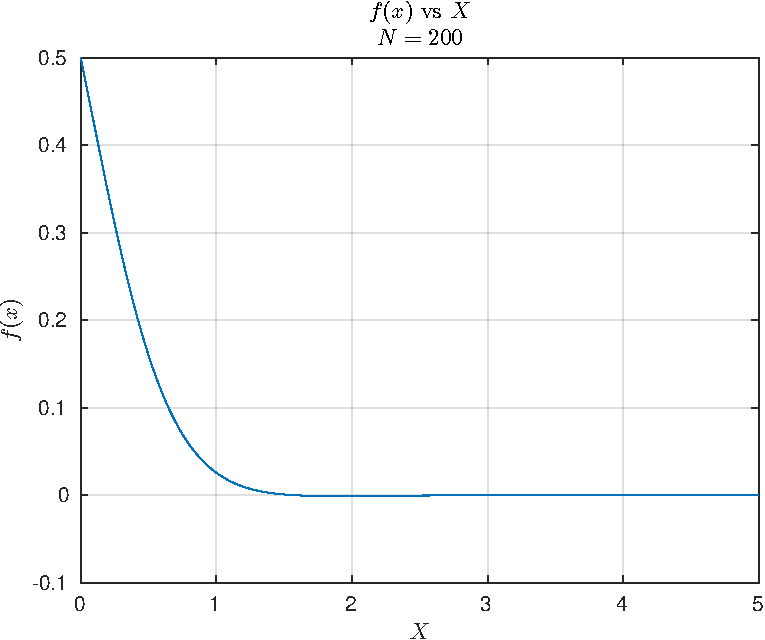
\includegraphics[width=1\linewidth]{Code/Fig/fx_200.pdf}
				\caption{\Large $f(x_{i}) = \frac{cos(x_{i})}{1 + e^{3x_{i}}}$ for $N \ = \ 200$}
				\label{fig:fx200}
			\end{figure}
			
			%%% Insert Figure Here as a .pdf File %%%
			\begin{figure}[H]
				\centering
				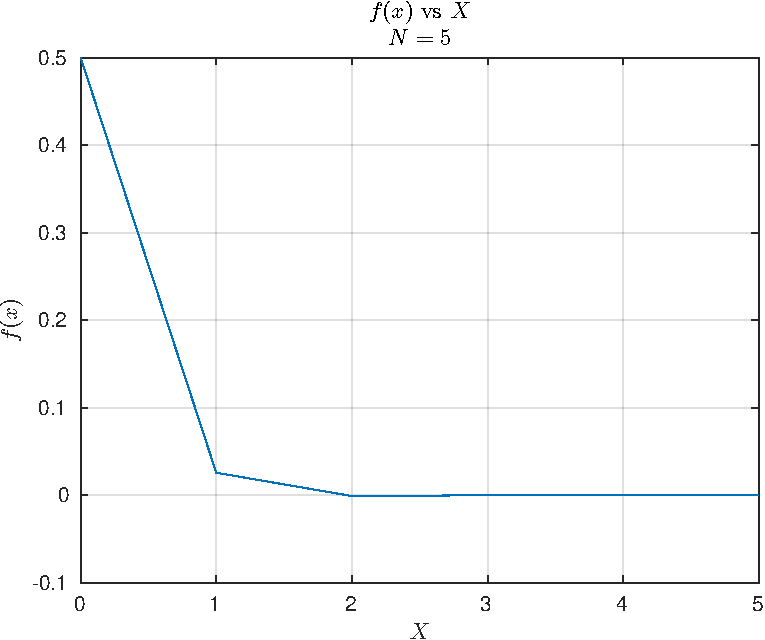
\includegraphics[width=1\linewidth]{Code/Fig/fx_5.pdf}
				\caption{\Large $f(x_{i}) = \frac{cos(x_{i})}{1 + e^{3x_{i}}}$ for $N \ = \ 5$}
				\label{fig:fx5}
			\end{figure}
			
			%%% Insert Figure Here as a .pdf File %%%
			\begin{figure}[H]
				\centering
				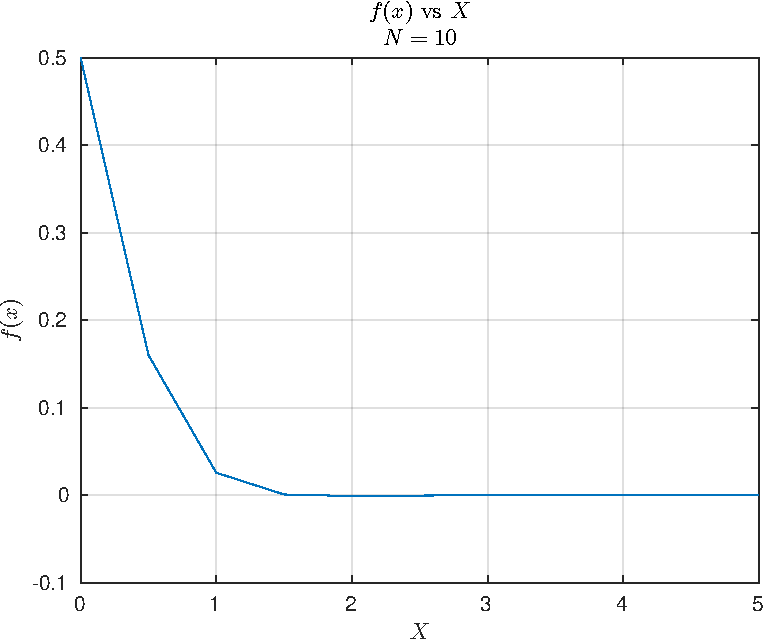
\includegraphics[width=1\linewidth]{Code/Fig/fx_10.pdf}
				\caption{\Large $f(x_{i}) = \frac{cos(x_{i})}{1 + e^{3x_{i}}}$ for $N \ = \ 10$}
				\label{fig:fx10}
			\end{figure}
			  Increasing the number of points (N+1) within the fixed sized region [0,5] for x decreases
			  the space between points, which enhances the resolution. Figure \ref{fig:fx200} exhibits a high domain resolution, resulting in a smooth and continuous plot devoid of discernible edges. Figures \ref{fig:fx5} and \ref{fig:fx10} conversely, demonstrate the effects of a lower domain resolution, characterized by visually apparent edges and a less refined plot appearance. 
			
	\section {Area under the Curve}
		\subsection{Standard Integration}
			%%% INSERT CODE HERE AS A .m FILE %%%
			\lstinputlisting[language=Matlab, caption = {\Large $\int_{0}^{5} \frac{cos(x)}{1 + e^{3x}} dx$}]{Code/integral.m}
			\begin{center}
				\LARGE $\int_{0}^{5} \frac{cos(x)}{1 + e^{3x}} dx \approx 0.201$
			\end{center}
			
		\subsection{Riemann Integral Approximation Equations}
			\subsubsection{Right Rectangular Approximation}
				%%% INSERT CODE HERE AS A .m FILE %%%
				\lstinputlisting[language=Matlab, caption = {\Large $\int_{0}^{5} \frac{cos(x)}{1 + e^{3x}} dx$}]{Code/q2.m}
				
				%%% Insert Figure Here as a .pdf File %%%
				\begin{figure}[H]
					\centering
					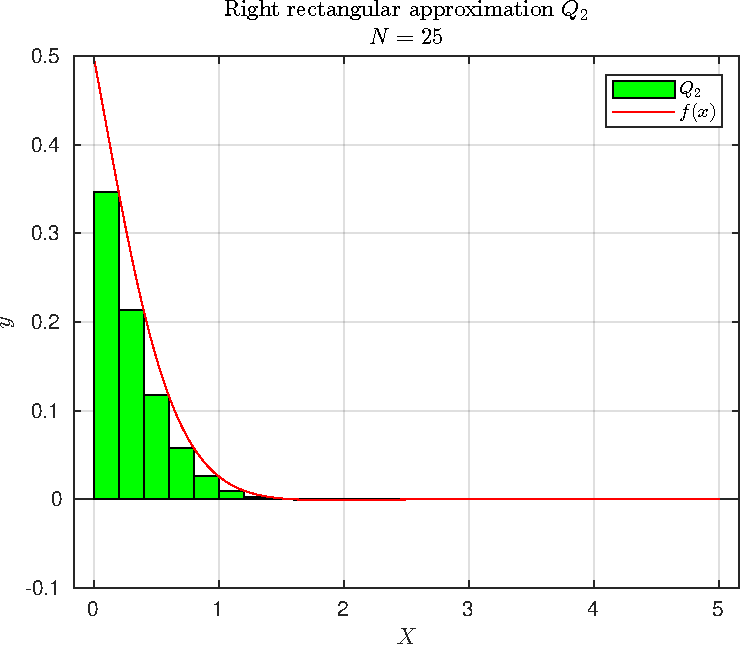
\includegraphics[width=1\linewidth]{Code/Fig/q2_bar_plot_25.pdf}
					\caption{\Large Right rectangular approximation for $Q_{2}$ for $N = 25$}
					\label{fig:q2barplot25}
				\end{figure}
			
				%%% Insert Figure Here as a .pdf File %%%
				\begin{figure}[H]
					\centering
					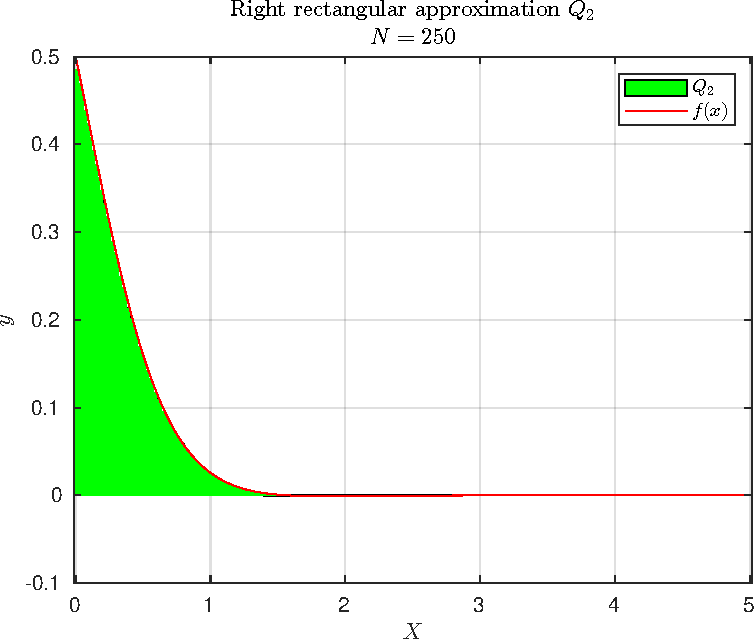
\includegraphics[width=1\linewidth]{Code/Fig/q2_bar_plot_250.pdf}
					\caption{\Large Right rectangular approximation for $Q_{2}$ for $N = 250$}
					\label{fig:q2barplot250}
				\end{figure}	
						
			\subsubsection{Tradeoffs}
			Deceasing $dx$ increases the resolution of the domain and the accuracy of the approximation. However, a higher resolution require more computational power. This is akin to higher resolution images requiring more space.
			\newpage
			\subsubsection{Trapazoidal approximation derivation}
				Given that the area of the first rectangle can be calculated:
				
				$$
				\begin{aligned}
					& f\left(x_{0}\right) d x_{0}+0.5\left(f\left(x_{1}\right)-f\left(x_{0}\right)\right) d x_{0} \\
					& f\left(x_{0}\right) d x_{0}+\frac{f\left(x_{1}\right)}{2} d x_{0}-\frac{f\left(x_{0}\right)}{2} d x_{0}
				\end{aligned}
				$$
				
				This means that the next area can be approximated:
				
				$$
				f\left(x_{1}\right) d x_{1}+\frac{f\left(x_{2}\right)}{2} d x_{1}-\frac{f\left(x_{1}\right)}{2} d x_{1}
				$$
				
				This can continue so forth until the $\mathrm{N}$-th area can be approximated as:
				
				$$
				f\left(x_{N-1}\right) d x_{N-1}+\frac{f\left(x_{N}\right)}{2} d x_{N-1}-\frac{f\left(x_{N-1}\right)}{2} d x_{N-1}
				$$
				
				Summing these terms up yields the equation $Q_{3}$
				
				$$
				Q_{3}=f\left(x_{0}\right) \frac{d x_{0}}{2}+\sum_{i=1}^{N-1} f\left(x_{i}\right) d x_{i}+f\left(x_{N}\right) \frac{d x_{N-1}}{2}
				$$
			\subsubsection{$Q_{3} = \frac{Q_{1} + Q_{2}}{2}$}				
				Given that:
				
				$$
				Q_{1}=\sum_{i=1}^{N-1} f\left(x_{i}\right) d x_{i}
				$$
				
				$$
				\begin{gathered}
					Q_{2}=\sum_{i=2}^{N} f\left(x_{i}\right) d x_{i-1} \\
					Q_{3}=f\left(x_{1}\right) \frac{d x_{1}}{2}+\sum_{i=2}^{N-1} f\left(x_{i}\right) d x_{i}+f\left(x_{N}\right) \frac{d x_{N-1}}{2}
				\end{gathered}
				$$
				
				All $d x_{i}$ are equal to each other. Substituting in $Q_{1}$ and $Q_{2}$ in to $Q_{3}$ gives:
				
				$$
				\begin{gathered}
					Q_{3}=\frac{1}{2}\left(\sum_{i=1}^{N-1} f\left(x_{i}\right) d x_{i}+\sum_{i=2}^{N} f\left(x_{i}\right) d x_{i-1}\right) \\
					Q_{3}=f\left(x_{1}\right) \frac{d x_{1}}{2}+\sum_{i=2}^{N-1} f\left(x_{i}\right) d x_{i}+f\left(x_{N}\right) \frac{d x_{N-1}}{2}
				\end{gathered}
				$$
			\newpage
			\subsubsection{$Q_{1}$ and $Q$ vs $N$}
				%%% INSERT CODE HERE AS A .m FILE %%%
				\lstinputlisting[language=Matlab, caption = {\Large $Q_{1}$ Function}]{Code/q1_sum.m}
				%%% INSERT CODE HERE AS A .m FILE %%%
				\lstinputlisting[language=Matlab, caption = {\Large Plot $Q_{1}$ and $Q$ vs $N$}]{Code/q1_plot.m}
				
				%%% Insert Figure Here as a .pdf File %%%
				\begin{figure}[H]
					\centering
					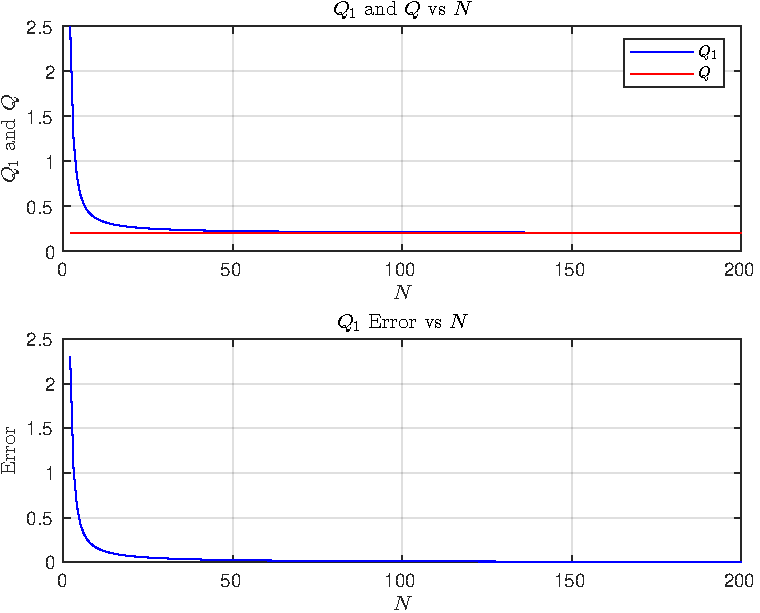
\includegraphics[width=1\linewidth]{Code/Fig/q1_sum_error_plot.pdf}
					\caption{\Large $Q_{1}$ and $Q$ vs $N$ and the \% Error for $Q_{1}$}
					\label{fig:q1sumerrorplot}
				\end{figure}	
				 $Q_{1}$ in Figure \ref{fig:q1sumerrorplot} converges to $Q$ at around $N \ \approx \ 75$	
				 \newpage
			\subsubsection{$Q_{3}$ and $Q$ vs $N$}
				%%% INSERT CODE HERE AS A .m FILE %%%
				\lstinputlisting[language=Matlab, caption = {\Large $Q_{3}$ Function}]{Code/q3_sum.m}
				%%% INSERT CODE HERE AS A .m FILE %%%
				\lstinputlisting[language=Matlab, caption = {\Large Plot $Q_{3}$ and $Q$ vs $N$}]{Code/q3_plot.m}
				
				%%% Insert Figure Here as a .pdf File %%%
				\begin{figure}[H]
					\centering
					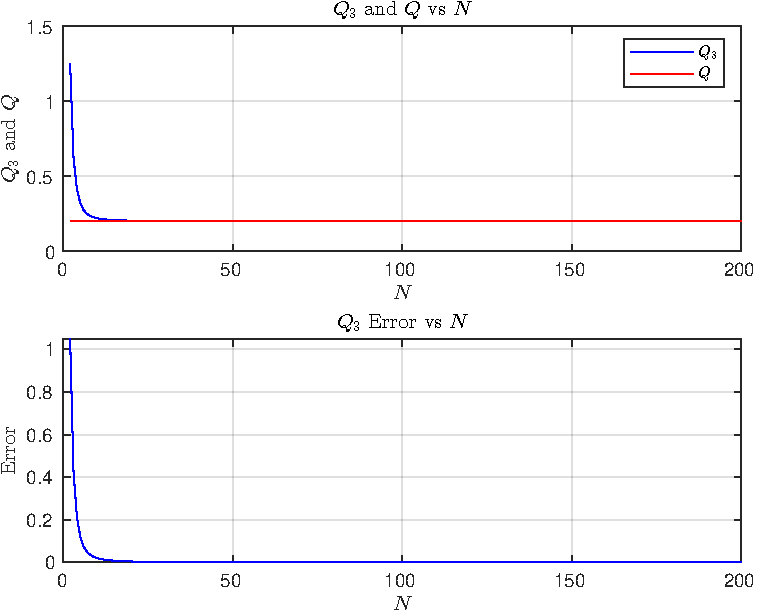
\includegraphics[width=1\linewidth]{Code/Fig/q3_sum_error_plot.pdf}
					\caption{\Large $Q_{3}$ and $Q$ vs $N$ and the \% Error for $Q_{2}$}
					\label{fig:q2sumerrorplot}
				\end{figure}
				
				%%% Insert Figure Here as a .pdf File %%%
				\begin{figure}[H]
					\centering
					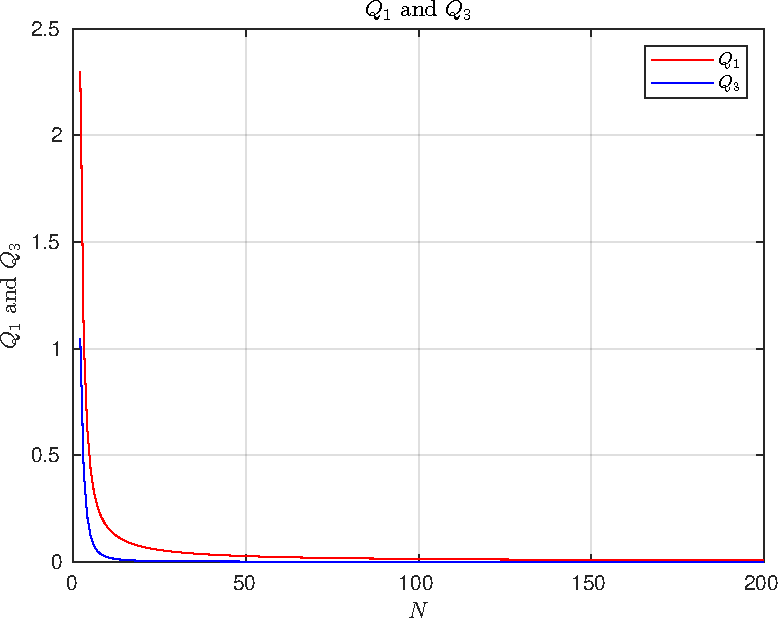
\includegraphics[width=1\linewidth]{Code/Fig/q1_q3_error_plot}
					\caption{\Large Error Comparison of $Q_{1}$ and $Q_{3}$}
					\label{fig:q1q3errorplot}
				\end{figure}
				
				 $Q_{3}$ in Figure \ref{fig:q2sumerrorplot} converges to $Q$ at around $N \ = \ 25$.
				 $Q_{3}$ converges to $Q$ at a faster rate compared to $Q_{1}$ as shown in Figure \ref{fig:q1q3errorplot}.
				 
	\section{Conclusion}
		%%% PUT CONCLUSION HERE %%
		This laboratory exercise showcases MATLAB's versatility across diverse scientific and engineering domains. It notably highlights the fundamental concept of trade-offs in engineering. Riemann summation serves as a poignant example, empowering students to grapple with the delicate balance between accuracy and computational efficiency: a fundamental skill for effective engineering design.
\end{document}